\section{Test-driven Development}

%-----------------------    ---------------------------------

\begin{frame}
\frametitle{}

\begin{center}
  
\includegraphics[width=12cm]{figs/validacion-contrasenas-TDD.png}
\end{center}


\begin{flushright}
{\tiny
Source: \url{http://inside.runroom.com/wp-content/uploads/2015/04/validacion-contrasenas-TDD.png}
}
\end{flushright}

\end{frame}


%-----------------------    ---------------------------------

\begin{frame}
\frametitle{El círculo del TDD}

\begin{center}
  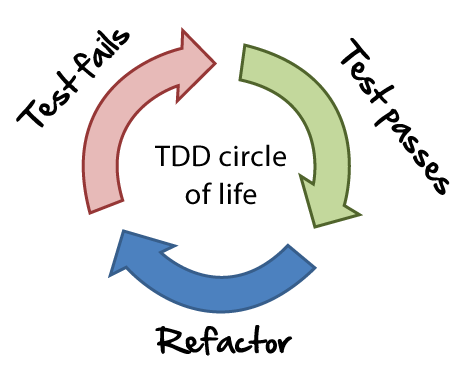
\includegraphics[width=9cm]{figs/tdd-circle-of-life.png}
\end{center}


\begin{flushright}
{\tiny
Source: \url{https://leantesting-wp.s3.amazonaws.com/resources/wp-content/uploads/2015/02/tdd-circle-of-life.png}
}
\end{flushright}

\end{frame}

%-----------------------    ---------------------------------

\begin{frame}[fragile]
\frametitle{Ejemplo de un test}


\begin{footnotesize}
\begin{verbatim}
newTest("Test the adding of two numbers").Execute = function () {
  var calc = {};
  calc.add = function () {
  }
  this.AreEqual(2, calc.add(1,1), "One plus one should equal two");
}
\end{verbatim}
\end{footnotesize}

\end{frame}

%-----------------------    ---------------------------------

\begin{frame}
\frametitle{Utilizando un framework}

\begin{center}
  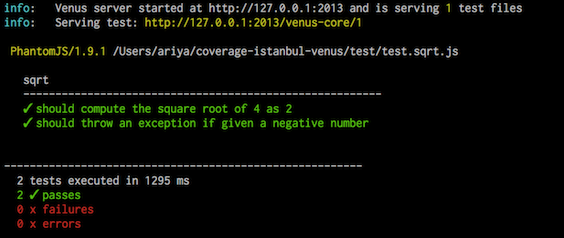
\includegraphics[width=12cm]{figs/venusjs.png}
\end{center}


\begin{flushright}
{\tiny
Source: \url{http://ariya.ofilabs.com/wp-content/uploads/2014/04/venusjs.png}
}
\end{flushright}

\end{frame}



%-----------------------    ---------------------------------

\begin{frame}
\frametitle{Frameworks para TDD en JavaScript}

\begin{itemize}
   \item QUnit 
   \item Jasmine
   \item Sinon
   \item TestSwarm
   \item Karma y Protactor
   \item ... y muchas más
\end{itemize}

\end{frame}

